\documentclass[dvipdfmx]{beamer}
\usepackage[absolute,overlay]{textpos}
\usepackage{graphicx}
\usepackage{url}
\usepackage{amsmath}
\usetheme{PaloAlto}

\newcommand{\tbs}{$\backslash$}

\title{TeX勉強会}
\author{RCC}
\date{令和元年~8月~5日}

\begin{document}
  \section{Title~Slide}
  \begin{frame}
    \centering
    {\Huge \bf TeX勉強会}\\
    令和元年~8月~5日
    \begin{figure}[h]
      \centering
      
\includegraphics[width=3cm]{images/iconRCC.png}
    \end{figure}
  \end{frame}
  \section{はじめに}
  \begin{frame}{はじめに}
    \Large
    \underline{\TeX とは?}
    \begin{itemize}
      \item {\scriptsize \TeX はアメリカ合衆国の数学者・計算機科学者であるドナルド・クヌースにより開発されている組版処理システムである。(Wiki調べ)}
      \item {\scriptsize バグが少ないソフトウェアとしても有名であり,テキストファイルを読み込むことで文章を組版し,DVI形式のファイルに書き出すことができる.}
    \end{itemize}
    \underline{\LaTeX とは?}
    \begin{itemize}
      \item {\scriptsize \TeX のマクロパッケージの1つであり,一般的な文書記述に優れている.}
      \item {\scriptsize これを日本語対応せたものに,日本語LaTeX が,更にそれを縦組みに対応させたものにpLaTeXがある.}
    \end{itemize}
  \end{frame}
  \section{環境構築について}
  \begin{frame}{環境構築について}
    \Large
    \underline{LaTeXを使うための環境構築について}\\~\\
    {\large オフラインで作業を行う場合}
    \begin{enumerate}
      \item[$\rightarrow$] {\scriptsize それぞれのOSにあった環境を構築する}\\
                           {\scriptsize (今回は説明は省きます)}
    \end{enumerate}
    ~\\
    {\large オンラインでのみ作業を行う場合}
    \begin{enumerate}
      \item[$\rightarrow$]{\scriptsize Cloud~LaTeXなどを利用する}\\
    \end{enumerate}
  \end{frame}
  \section{Cloud LaTeXを使う}
  \begin{frame}{Cloud LaTeXについて}
    \Large
    \underline{Cloud LaTeXとは$\cdots$}\\~\\
    \begin{figure}[h]
      \centering
      
\includegraphics[width=8cm]{images/CloudLaTeX.png}
    \end{figure}
    \centering
    {\small ローカルで環境を構築せずとも,オンラインで\TeX が書けるサイト}\\
    {\small \url{https://cloudlatex.io/ja}}
  \end{frame}
  \begin{frame}{Cloud LaTeXに登録する}
    \small
    \begin{enumerate}
      \item {\scriptsize 前スライドのリンク先に飛び,以下のようなボタンをクリックする.}
            \begin{figure}[h]
              \centering
              
\includegraphics[width=2cm]{images/shinkitouroku.png}
            \end{figure}
      \item {\scriptsize 必要な情報を入力するか,FaceBookまたはTwitterのアカウントを利用して登録する.}
      \item {\small \bf 登録完了!!}
    \end{enumerate}
  \end{frame}
  \begin{frame}{プロジェクトを作成する}
    \begin{enumerate}
      \item {\scriptsize 画面左側の,新規プロジェクトを選択}
            \begin{figure}[h]
              \centering
              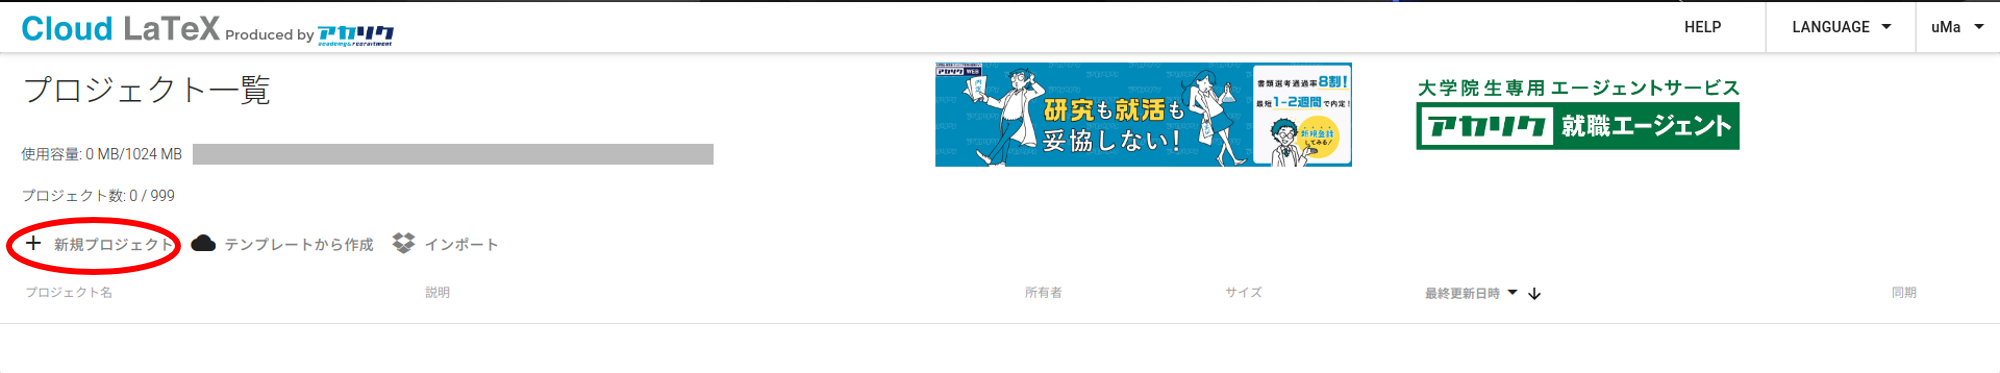
\includegraphics[width=9cm]{images/CreateProject1.png}
            \end{figure}
      \item {\scriptsize 以下のようなウィンドウが出てくるので,プロジェクト名と説明の欄を記入して,作成を選択}
            \begin{figure}[h]
              \centering
              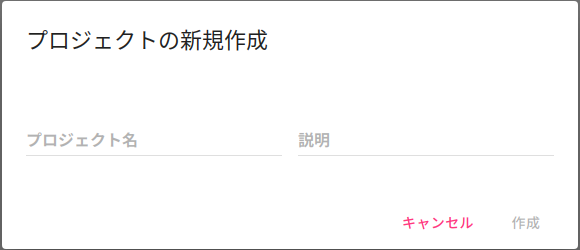
\includegraphics[width=3cm]{images/CreateProject2.png}
            \end{figure}
      \item {\scriptsize すると,以下のようにプロジェクトが追加される.}
            \begin{figure}[h]
              \centering
              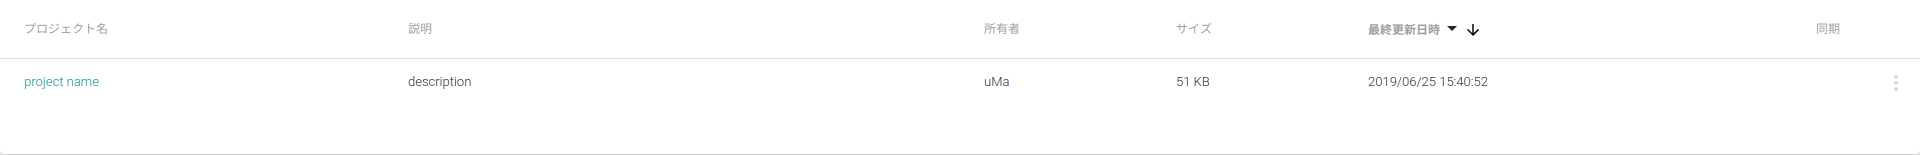
\includegraphics[width=9cm]{images/CreateProject3.png}
            \end{figure}
    \end{enumerate}
  \end{frame}
  \begin{frame}{プロジェクトを編集する}
    \begin{enumerate}
      \item {\scriptsize 編集したいプロジェクト名の部分をクリックする}
            \begin{figure}[h]
              \centering
              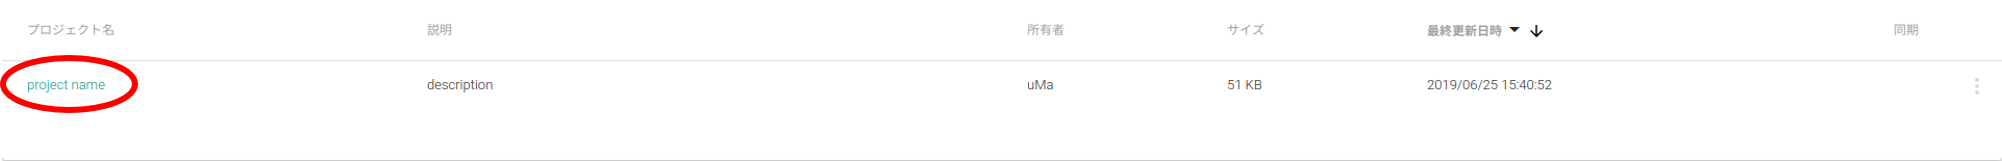
\includegraphics[width=9cm]{images/EditingProject1.png}
            \end{figure}
      \item {\scriptsize 以下のようなページが開くので,そこで編集を行う}
            \begin{figure}[h]
              \centering
              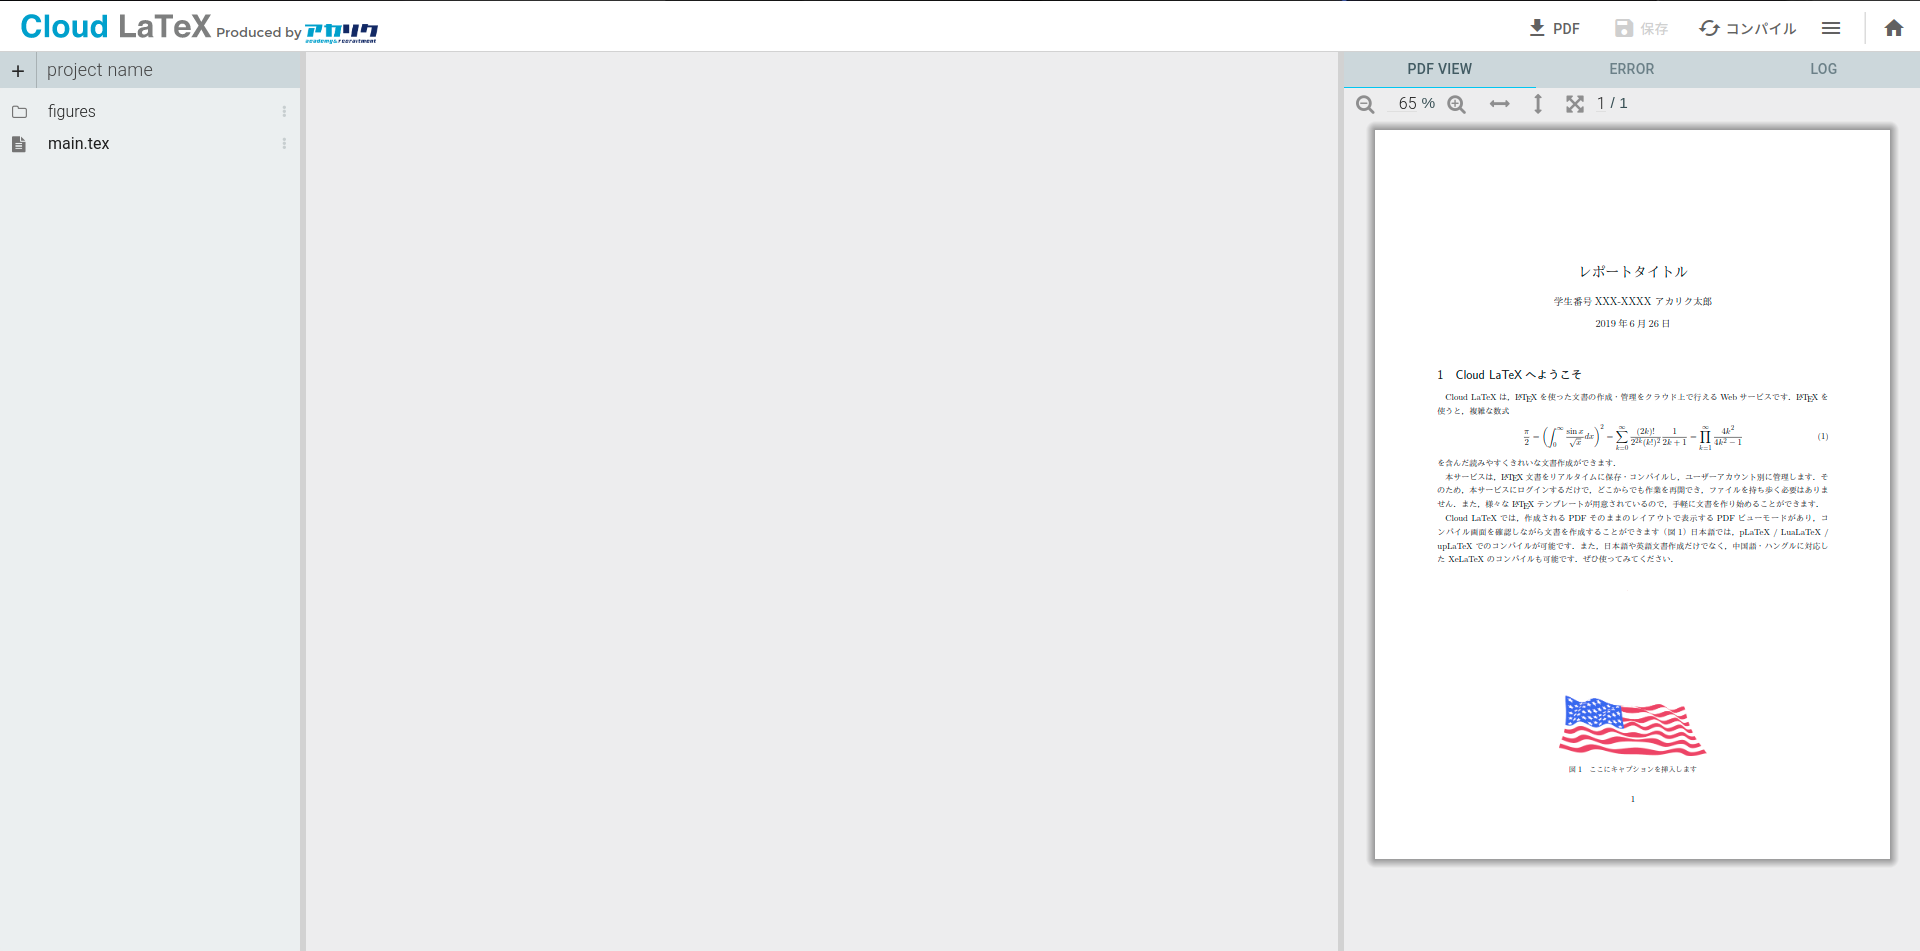
\includegraphics[width=9cm]{images/EditingProject2.png}
            \end{figure}
    \end{enumerate}
  \end{frame}
  \begin{frame}{編集画面の説明}
    \begin{figure}[h]
      \centering
      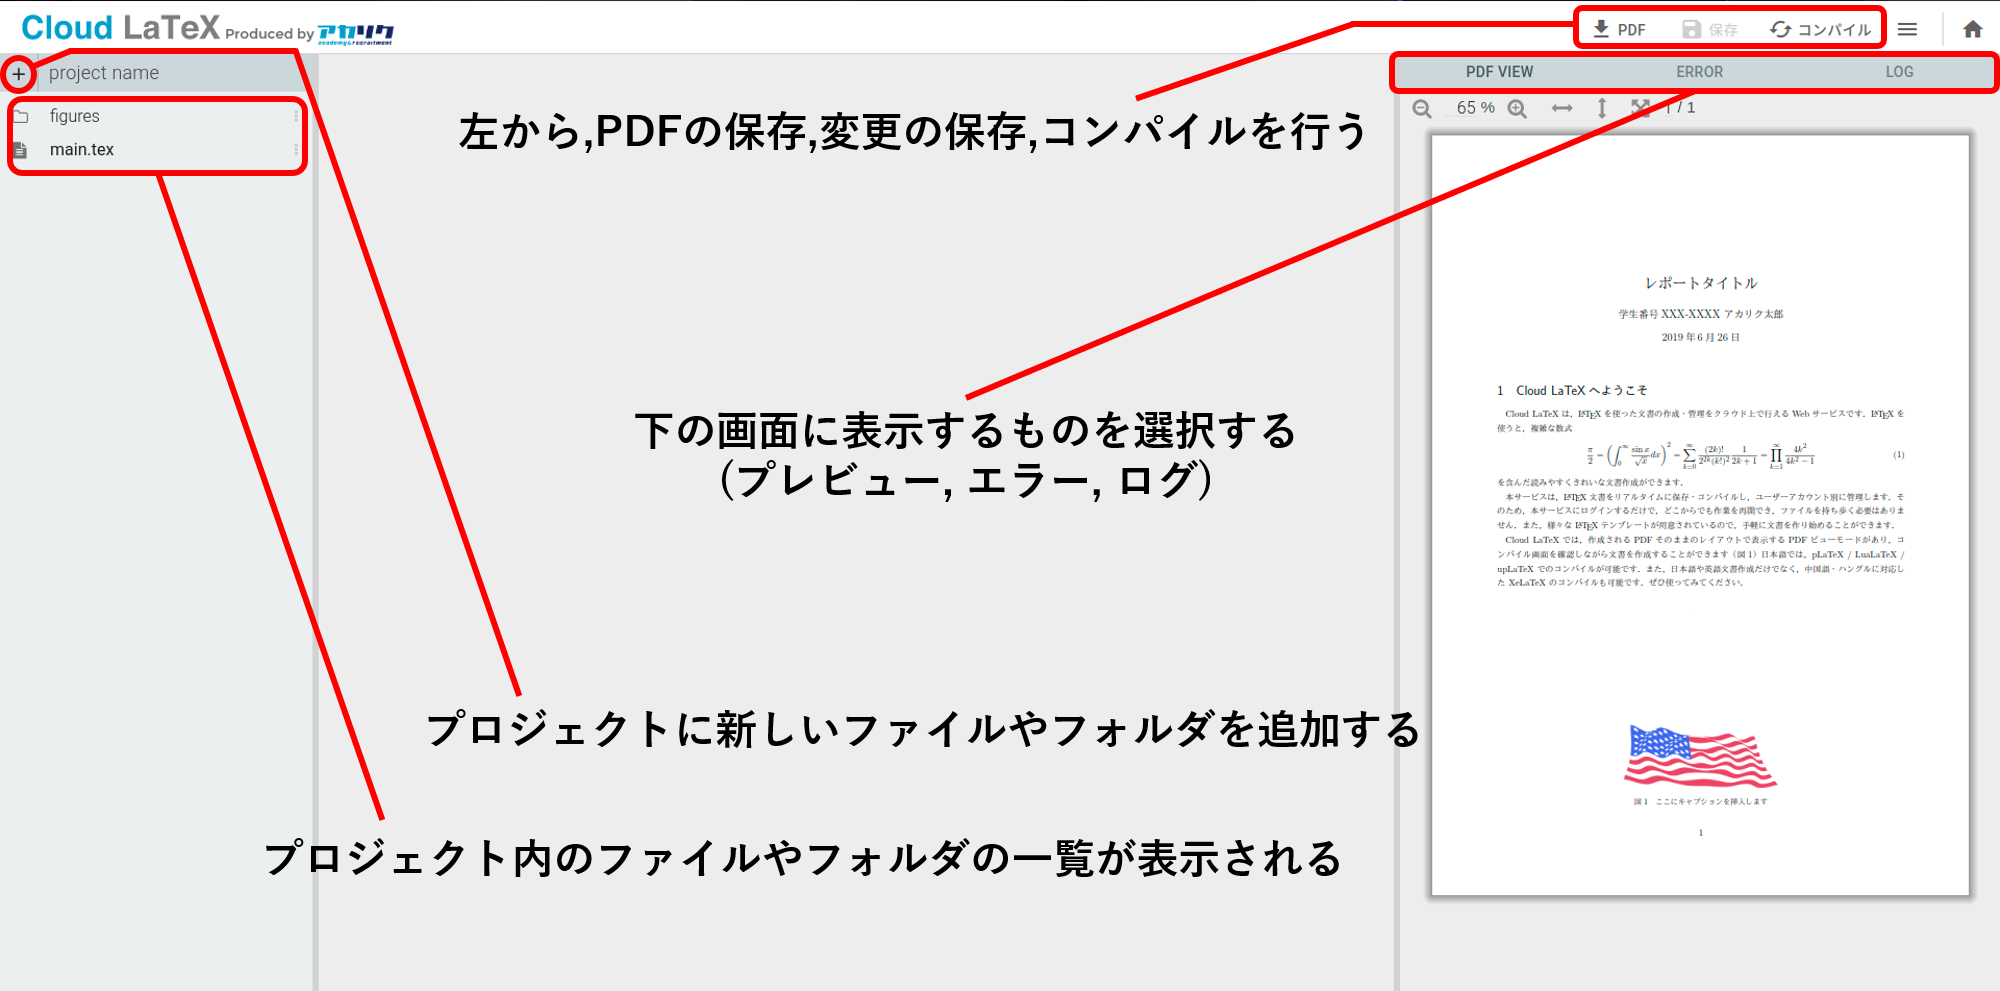
\includegraphics[width=10cm]{images/IntroductionOfEditing.png}
    \end{figure}
    {\scriptsize *右上の三本線のアイコンから,各種設定をすることもできる}\\
    {\scriptsize *同じく右上のホームアイコンをクリックすると,ホーム画面に戻ることができる}\\
    {\scriptsize *左側に表示されているmain.texをクリックして,ファイルを開いてみましょう}
  \end{frame}
  \section{\LaTeX で書く}
  \begin{frame}{\LaTeX で書く}
    \centering\Huge\bf
    実際に書いてみましょう
  \end{frame}
  \begin{frame}{基本的な構成}
      どのような文書にするのかどうかを設定する\\~\\
      {\scriptsize
      \tbs documentclass[オプション]\{文書クラス\}\\
      \begin{itemize}
        \item オプションでは,文字サイズや用紙のサイズを指定する\\
              {\tiny 例. [12pt, a4paper]}\\~\\
        \item 文書クラスでは,どのような文書を書くのかを指定する\\
              {\tiny 例. article, jarticle, jbook, jreport}\\~\\
      \end{itemize}
      }
      パッケージを利用する\\~\\
      {\scriptsize
      \tbs usepackage[オプション]\{パッケージ名\}
      \begin{itemize}
        \item オプションはない場合もある(また,指定しないこともできる)\\~\\
        \item パッケージは,必要なものを利用する.~Cloud LaTeXでは,ある程度有名なパッケージは
              使えるようになっている.(usepackageの記述は必要)
      \end{itemize}
      }
  \end{frame}
  \begin{frame}{基本的な構成}
    \LaTeX のコマンドは大きく分けて2種類
    \scriptsize
    \begin{itemize}
      \item \tbs begin\{命令名\}ここに命令を適用させたいスクリプト\tbs end\{命令名\}\\~\\
      \item \tbs 命令名~で,命令を適用する\\~\\~\\
    \end{itemize}
    \scriptsize
    本文は,\\~\\
    \tbs begin\{document\}\\
    本文\\
    \tbs end\{document\}\\~\\
    のように記述する.\\
    \tbs end\{document\}以降に記述しても反映されないので注意
  \end{frame}
  \begin{frame}{タイトルを作る}
    \bf
    \tbs maketitleを使うと,自動的にタイトルを生成してくれる\\~\\~\\
    \scriptsize
    \tbs maketitleを使用する前に以下を記述しておく必要がある\\~\\
    \begin{itemize}
      \item \tbs title\{タイトル\}\\~\\
      \item \tbs author\{著者名\}\\~\\
      \item \tbs date\{日付\}
    \end{itemize}
    ~\\~\\~\\
    タイトルページと本文を分けたい場合は,\tbs newpageを用いて,次のページに移行する.
  \end{frame}
  \begin{frame}{文字サイズを変更する}
    文字サイズは,以下のようなコマンドで変更することができる.
    \begin{table}[h]
      \scriptsize
      \begin{tabular}{|l|c|}\hline
        コマンド&サイズ \\ \hline
        \tbs tiny&{\tiny 世の中には(5pt)} \\ \hline
        \tbs scriptsize&世の中には(7pt) \\ \hline
        \tbs small&{\small 世の中には(9pt)} \\ \hline
        \tbs normalsize & {\normalsize 世の中には(10pt)}\\ \hline
        \tbs large&{\large 世の中には(12pt)} \\ \hline
        \tbs Large&{\Large 世の中には(14.4pt)} \\ \hline
        \tbs huge&{\huge 世の中には(20.74pt)} \\ \hline
      \end{tabular}
    \end{table}
    {\scriptsize *他にも,\tbs footnotesize(8pt)や,\tbs LARGE(17.28pt), \tbs Huge(24.88pt)がある.}\\
    {\scriptsize *\tbs fontsize\{フォントサイズ\}\{行送り\}を用いて細かく指定することもできる.}\\
    {\scriptsize *\tbs bfで{\bf Bold Font}にすることができる}\\
    {\scriptsize *\{\tbs large\tbs bf~この中に書かれた文章だけlargeのサイズの{\bf Bold Fontになる}\}}
  \end{frame}
  \begin{frame}{特殊な文字などを挿入する}
    \begin{center}
      スクリプトに書いても直接反映されない文字や,\\
      特殊な記号は,コマンドを利用して挿入することができる.
    \end{center}
    \begin{table}[h]
      \scriptsize
      例.特殊文字と,それを表示するためのコマンド\\
      \centering
      \begin{tabular}{|c|c|} \hline
        コマンド&表示される文字 \\ \hline
        \tbs \&&\& \\ \hline
        \tbs textbar&\textbar \\ \hline
        \tbs \{&\{ \\ \hline
        \tbs \}&\} \\ \hline
        \tbs alpha&$\alpha$ \\ \hline
        \tbs beta &$\beta$ \\ \hline
      \end{tabular}
    \end{table}
    ~\\
    {\scriptsize *空白は\~{}で,改行は\tbs\tbs で行うことができる.}\\
    {\scriptsize *他にも様々なコマンドがある.}\\
    {\scriptsize *$\alpha$,$\beta$は後のスライドで説明する{\bf 数式モード}内で使用する}\\
    {\scriptsize *\%を記述した行では,それ以降がコメントとされる.}
  \end{frame}
  \begin{frame}{箇条書きをする}
    itemize環境,enumerate環境で箇条書きをすることができる.
    \scriptsize
    \begin{itemize}
      \item itemize環境\\
            itemize環境を使用すると,記号(・)がitemの左側につく.\\
            改行は,itemの直前に自動的に行われる.\\~\\
            \begin{table}[h]
              \centering
              \tbs begin\{itemize\}\\
              ~~~~\tbs item~項目1\\
              ~~~~\tbs item~項目2\\
              \tbs end\{itemize\}\\~\\
            \end{table}
      \item enumerate環境\\
            enumerate環境を用いると,番号が1から順にitemの左側につく.\\
            改行はitemizeと同じく自動的に行われる.\\~\\
            \begin{table}[h]
              \centering
              \tbs begin\{enumerate\}\\
              ~~~~\tbs item~項目1\\
              ~~~~\tbs item~項目2\\
              \tbs end\{enumerate\}
            \end{table}
    \end{itemize}
  \end{frame}
  \begin{frame}{箇条書きをする}
    \begin{center}
      決められたラベル(・や番号など)ではなく,\\
      指定したラベルをつけて箇条書きにすることもできる
    \end{center}
    \scriptsize
    \begin{itemize}
      \item description環境を用いると,指定したラベルがitemの左側につく.\\~\\
    \end{itemize}
    \begin{table}[h]
      \centering
      \tbs begin\{description\}\\
      ~~~~\tbs item[label] 項目\\
      ~~~~\tbs item[label] 項目\\
      \tbs end\{description\}
    \end{table}
    ~\\~\\
  \end{frame}
  \begin{frame}{数式を挿入する}
    \LaTeX では,数式モードという数式を埋め込む方法が存在する\\~\\
    \scriptsize
   {\normalsize\bf インライン数式モード(以下の3つは実行結果が同じ)}
    \begin{enumerate}
      \item \$数式\$\\~\\
      \item \tbs (数式\tbs )\\~\\
      \item \tbs begin\{math\}数式\tbs end\{math\}\\~\\~\\
    \end{enumerate}
    {\normalsize\bf ディスプレイ数式モード}
    \begin{itemize}
      \item \tbs[数式\tbs]\\~\\~\\
    \end{itemize}
    {\normalsize\bf 番号付きディスプレイ数式モード}
      \begin{itemize}
        \item \tbs begin\{equation\}数式\tbs end\{equation\}
      \end{itemize}
  \end{frame}
  \begin{frame}{数式を挿入する}
    複数行の数式を挿入する場合\\~\\
    \scriptsize
    {\normalsize\bf eqnarrayを使う}\\
    {\tiny 以下のコマンドは,合わせたい位置を\&\&で囲むことで,複数行の数式を挿入することができる.}
    \begin{itemize}
      \item \tbs begin\{eqnarray\}数式\tbs\tbs 数式$\cdots$\tbs end\{eqnarray\}\\
            (この場合,全ての行の式に番号が振られる)\\~\\
      \item 改行をする前に,\tbs nonumberと記述することで,その行の式の数式番号を割り振らない
            ことができる.\\~\\
      \item eqnarray*とすることで,番号の割り振りを無効にすることができる.\\~\\
    \end{itemize}
    例.\\
    \begin{center}
      \tbs begin\{eqnarray*\}\\
      ~~~~f(x)~\&=\&~x+x\\
      ~~~~\&=\&2x\\
      \tbs end\{eqnarray*\}
    \end{center}
  \end{frame}
  \begin{frame}{数式を挿入する}
    \underline{数式内でよく使う表記の記述方法}\\
    \scriptsize
    \begin{table}[h]
      \centering
      \begin{tabular}{|c|c|}\hline
        コマンド&表示される文字 \\ \hline
        x\^{}\{n\}&$x^{n}$ \\ \hline
        x\_\{n\}&$x_{n}$ \\ \hline
        \tbs frac\{a\}\{b\} & $\frac{a}{b}$ \\ \hline
        \tbs int\^{}\{a\}\_\{b\} & $\int_{a}^{b}$ \\ \hline
        \tbs sum\^{}\{a\}\_\{b\} & $\sum^{a}_{b}$ \\ \hline
      \end{tabular}
    \end{table}
    ~\\~\\
    また,数式を扱う上で,amsmathという便利なパッケージがある.\\
    amsmathを使用すると,以下のような表示などができるようになる.詳しくはamsmathで検索.\\
    \[
    u(x)=
    \begin{cases}
      1 & (x\ge0)\\
      0 & (x<0)
    \end{cases}
    \]
  \end{frame}
  \begin{frame}{表を作成する}
    table環境とtabular環境を用いて,表を作成することができる\\~\\
    \scriptsize
    例.\\
    \centering
    \begin{minipage}[c]{4cm}
    \tbs begin\{table\}[位置の指定]\\
    ~~\tbs begin\{tabular\}\{列の指定\}\\
    ~~~~表の中身\\
    ~~\tbs end\{tabular\}\\
    \tbs end\{table\}
  \end{minipage}
  ~\\~\\~\\
  \begin{minipage}[c]{5cm}
    \begin{table}
      \centering
      tabularの位置の指定
      \begin{tabular}{|c|l|} \hline
        位置&出力方法 \\ \hline
        h&その場所に表を挿入する \\ \hline
        t&ページ上端に表を挿入 \\ \hline
        b&ページ下端に表を挿入 \\ \hline
        p&専用ページを作成して挿入 \\ \hline
      \end{tabular}
    \end{table}
  \end{minipage}
  \begin{minipage}[c]{5cm}
    \begin{table}[h]
      \centering
      列の指定方法
      \begin{tabular}{|c|l|} \hline
        列指定&表示位置 \\ \hline
        l&左に寄せて表示 \\ \hline
        c&真ん中に表示 \\ \hline
        r&右に寄せて表示 \\ \hline
      \end{tabular}
    \end{table}
  \end{minipage}
  \end{frame}
  \begin{frame}{表を作成する}
    \scriptsize
    列の指定をするときに,$\mid$c$\mid$c$\mid$のように縦線を入れて指定することで,
    その要素と要素の間に縦線を表示することができる.\\~\\
    改行する前に\tbs hlineを入れることで,列の下に横線を引くことができる.\\~\\
    例.\\~\\
    \centering
    \begin{minipage}[h]{4cm}
      \tbs begin\{table\}[h]\\
      ~~\tbs begin\{tabular\}\{ccc\}\\
      ~~~~\~{}\&2\&4~\tbs\tbs\\
      ~~~~\~{}\&3\&4~\tbs\tbs~\tbs hline\\
      ~~~~+\&5\&8\\
      ~~\tbs end\{tabular\}\\
      \tbs end\{table\}
    \end{minipage}
    \begin{minipage}[h]{4cm}
      \tbs begin\{table\}[h]\\
      ~~\tbs begin\{tabular\}\{$\mid$c$\mid\mid$c$\mid$c$\mid$\}\tbs hline\\
      ~~~~1\&2\&3~\tbs\tbs~\tbs hline\tbs hline \\
      ~~~~4\&5\&6~\tbs\tbs~\tbs hline \\
      ~~~~7\&8\&9~\tbs\tbs~\tbs hline \\
      ~~\tbs end\{tabular\}\\
      \tbs end\{table\}
    \end{minipage}
    ~\\~\\~\\~\\
    実際に上のような表を作成してみて下さい.
  \end{frame}
  \section{おまけ}
  \begin{frame}
    \centering\Huge\bf
    おまけ
  \end{frame}
  \begin{frame}{ファイルを分割する}
    \scriptsize
    \LaTeX では,文章が長くなり,コンパイル時間や,エラーの修正の手間も長くなってしまうことを
    防ぐために,ファイルを分割する機能が存在する.\\~\\
    \begin{itemize}
      \item {\normalsize\bf\tbs inputを使用する}\\
            \tbs input\{相対パス\}のようにして他のファイルを読み込むことができる.\\
            これを利用してファイルを分割する.\\~\\
      \item {\normalsize\bf\tbs includeを使用する}\\
            inputと同じように相対パスで指定したファイルを読み込むことができるが,
            コマンドの前後が改ページされる.
    \end{itemize}
  \end{frame}
  \begin{frame}{新しいコマンドを作成する}
    \Large\bf
    自分でマクロを定義することもできます
    \begin{itemize}
      \item {\scriptsize 引数を取らない場合}\\
        {\scriptsize \tbs newcommand\{\tbs 定義するマクロ名\}\{定義の本体部分\}}\\
        {\tiny 例.\tbs newcommand\{\tbs eru\}\{スノー・ホワイト・パラダイス・エルサント・フロウ・ワスレナ・ピュア・プリンセス・リーブル・ラブ・ハイデルン・ドコドコ・ヤッタゼ・ヴァルキュリア・パッション・アールヴ・ノエル・チャコボシ・エルアリア・フロージア・メイドイン・ブルーム・エル\}}
      \item {\scriptsize 引数を取る場合}\\
        {\scriptsize \tbs newcommand\{\tbs 定義するマクロ名\}[引数の数]\{定義の本体部分\}}
        {\tiny 例.\tbs newcommand\{\tbs integ\}[2]\{\tbs int\_\{\#1\}\textasciicircum\{\#2\}\}}\\
        {\tiny ~~~~~\tbs integ\{-\tbs infty\}\{\tbs infty\}~$\rightarrow$~$\int_{-\infty}^{\infty}$}
    \end{itemize}
  \end{frame}
  \begin{frame}{スライドを作成する}
    \begin{center}
      \Large\bf
      実はこのスライド,\LaTeX で書いてます~\\~\\
    \end{center}
    \begin{itemize}
      \item beamerというパッケージを使えばスライドを作成することができる
      \item 数式や表の挿入が簡単であるため,発表の内容によっては向いているものもある
      \item 位置の調整も,慣れればきれいにできる
    \end{itemize}
  \end{frame}
  \begin{frame}{その他}
    その他便利なパッケージや環境など\\~\\
    \scriptsize
    \begin{itemize}
      \item {\normalsize\bf amsmath}\\
            数式を扱うための便利な環境が用意されているパッケージ.\\~\\
      \item {\normalsize\bf graphicx}\\
            includegraphicsなどのコマンドが使用できる.画像の挿入などに使用する.\\~\\
      \item {\normalsize\bf minipage環境}\\
            minipage環境を用いることによって,ページを分割したり,画像,表を並べて表示することができる.
    \end{itemize}
  \end{frame}
  \section{おわり}
  \begin{frame}{おわり}
    \centering\Large\bf
    ご清聴ありがとうございました
  \end{frame}
\end{document}
